\documentclass[10pt,a4paper]{article}

\usepackage[T1]{fontenc}
\usepackage[utf8]{inputenc}
\usepackage[margin=1.8cm]{geometry}
\usepackage{amsmath}
\usepackage{booktabs}
\usepackage{graphicx}
\usepackage{microtype}

\setlength{\parskip}{0pt}
\linespread{0.94}\selectfont
\renewcommand{\topfraction}{0.95}
\renewcommand{\bottomfraction}{0.95}
\renewcommand{\textfraction}{0.04}
\renewcommand{\floatpagefraction}{0.9}
\setcounter{topnumber}{2}
\setlength{\textfloatsep}{8pt plus 2pt minus 2pt}
\setlength{\intextsep}{8pt plus 2pt minus 2pt}
\renewcommand{\arraystretch}{1.05}

\title{\vspace{-1.3cm}\textbf{X-ray properties of Galactic HMXBs corrected\\ by interstellar absorption}}
\author{Marina Belén Badaracco \\[2pt]
\normalsize Professors: Dr.\ Matías Zaldarriaga \ \& \ Dr.\ Nahuel Miron Granese \\[2pt]
\normalsize \textit{Assistant: Claude Code 2.1.278, Opus 5, effort high}}
\date{28 September 2026}

\begin{document}
\maketitle
\vspace{-0.9cm}

\section{Introduction}

Two recent catalogues define the observational state of Galactic high-mass
X-ray binaries (HMXBs). Fortin et al.\ (2023, hereafter F23) compile 152 systems
with 111 \textit{Gaia}~DR3 counterparts and Bailer-Jones et al.\ (2021)
distances, but tabulate \emph{no} X-ray flux, column density or spectral slope.
Neumann et al.\ (2023) give 169 systems with fluxes in five bands and one column
density, taken from the \textit{Swift} catalogue, where it came from
interpolating a power law through hardness ratios rather than from a spectral
fit. For a population lying in the Galactic plane this is the gap that matters:
below about 2~keV an HMXB spectrum is shaped more by absorption than by
emission.

The column measured towards an HMXB is a sum: one part interstellar, the other
local, produced by the donor's wind, the accretion stream and the photoionised
wake trailing the compact object. Only the second is a property of the binary.
Doroshenko et al.\ (2024) make the separation possible with a pan-Galactic
cumulative-reddening cube, calibrated against independent X-ray absorption
measurements and distributed with $E(B-V)\rightarrow N_{\rm H}$ conversions:
queried at the Bailer-Jones distance it returns the interstellar column, and the
remainder of a fitted $N_{\rm H}$ is the local one. The subtraction cannot be
done with point values --- the distance has an asymmetric posterior, the cube its
own calibration uncertainty, the conversion depends on the abundance table ---
so the interstellar column must be drawn as a distribution and a Monte Carlo
over distance, cube and conversion is required for the residual to have an
honest error bar.

The local column is not a constant of the system. In a wind-fed HMXB the compact
object moves through an inhomogeneous, ionised outflow, and the material along
the sight line changes around the orbit: it peaks near superior conjunction of
the compact object and drops near inferior conjunction. A time-averaged residual
mixes physically distinct states, and averaging over phase destroys the signal
that identifies the absorber. The aim is not one number per system but the run
of the local column \emph{with orbital phase}, measured homogeneously across the
sample. The systems without a usable phase are analysed for their column all the same,
and several may yet acquire one: the period is recoverable in principle by
folding our own light curves or from periodograms of the archival monitoring.

\section{Crossmatch}

The sample is built outwards from F23. Optical counterparts come from a
\textit{Gaia}~DR3 crossmatch whose acceptance is a statistical test and not a
fixed radius: it combines the developments of Pineau et al.\ (2011, 2017) and is
at bottom a $\chi^{2}$ test with two degrees of freedom, corrected for spherical
geometry. F23's 90\% positional errors are rescaled, \textit{Gaia}'s
milliarcsecond errors converted, the RA--Dec correlation retained, and a pair
accepted when $d_{M}^{2}<9.21$.

X-ray counterparts come from the two catalogues that supply spectra, CSC~2.1.1
and 5XMM-DR15, matched through their own positional errors. The working sample
is the \textbf{89 systems with at least one X-ray counterpart}:
61 with a CSC source, 60 with a 5XMM source and \textbf{32 with both} --- the
overlap that makes a cross-mission comparison possible at all. Every identification is recorded three ways, ours against F23's against SIMBAD's
(89/88/85, 61/53/46 and 60/58/53 respectively), each decision written into a
\texttt{Notes} column. A few systems also appear in the low-mass
X-ray binary catalogue of Fortin et al.\ (2024); those were found and treated
individually.

\textbf{Every X-ray counterpart F23 itself reports is also being analysed,
including the ones our crossmatch leaves out}: the two criteria are different
statistical statements about the same sky, and exclusion by ours is no
demonstration of non-detection.

\section{Homogenization I: re-reduction of \textit{Chandra} and \textit{XMM-Newton}}

The point of this stage is comparability between the missions, not agreement
with either catalogue. \textbf{CSC~2.1.1} fits an absorbed power law over
0.5--7.0~keV with a $\chi^{2}$ statistic, then collapses the contributing
observations with Bayesian Blocks, those outside the chosen block not entering
at all. \textbf{5XMM-DR15} reports
stacked columns fitted to five band count rates \emph{assuming each source's
flux is constant across all exposures}, and, separately, a spectral fit over
0.2--12~keV with the Cash statistic combining at most one pn and one MOS
detection. Neither source-level number is defined for a variable source, and
every system here is variable, so this work stays at the \emph{detection level}
throughout.

\paragraph{Why the catalogue columns cannot be used for this.} They are the
wrong kind of object for what follows. A catalogue publishes a best-fit
$N_{\rm H}$ and at most a 68\% interval; the \emph{probability distribution}
behind that number is not published --- neither its shape, strongly asymmetric
for a column bounded below at zero and fitted on few counts, nor its covariance
with $\Gamma$ and the normalisation. What this project wants is a difference:
the measured column minus an interstellar column that must itself be drawn as a
distribution. Subtracting a distribution from a point estimate with a symmetric
error bar does not propagate the error, it invents one, and the result is binned
in orbital phase, where the scatter between bins is the signal. The fits must
therefore be ours, made in XSPEC (Arnaud et al.\ 2025) with each posterior kept
rather than summarised.

\emph{Stage~1} reproduces each catalogue's own per-detection fit as validation:
105 of 115 \textit{Chandra} detections reach the published reduced statistic,
our $N_{\rm H}$ inside the published 68\% interval for 92 and $\Gamma$ for 98.
The reprocessing behind Stage~2 is complete.

Solar-flare screening, which builds the good time intervals, is deliberately
deferred. It derives them from a whole-field light curve above 10~keV meant to
trace the soft-proton background --- but a bright hard point source contributes
to that curve, and an HMXB is exactly that, variable on the same timescales.
Left in the field its own variability reads as background flaring, and the
intervals cut are exactly those in which it is brightest, the states this
project exists to measure. The bright sources must first be detected so that
they can be excluded from the region the curve is built on. That detection is
now complete.

\section{Homogenization II: orbital phases}

This is the part with no established recipe to follow, and it is what makes the
phase study possible at all.

F23 tabulates an orbital period for 72 of the 89 systems and \emph{no epoch
column whatsoever}. Phase zero had to be read by hand out of the literature,
one paper at a time, with the sentence or table row it came from recorded
beside it so that any entry can be rechecked without re-reading the paper. That
produced 57 epochs, and they are not the same kind of quantity: they fall into
ten conventions (Table~\ref{tab:t0}), from a periastron passage to an arbitrary
origin used to fold a light curve.

\begin{table}[t]
\centering
\footnotesize
\caption{The 57 published epochs, by what the paper says they are.}
\label{tab:t0}
\begin{tabular}{lcl}
\toprule
convention & $N$ & status \\
\midrule
periastron & 19 & already on the convention \\
outburst maximum, Be XB & 5 & \emph{is} a periastron passage \\
$T_{\pi/2}$ & 7 & convertible, needs $\omega$ \\
mid-eclipse & 5 & convertible, needs $\omega$ \\
superior conjunction & 4 & convertible, needs $\omega$ \\
inferior conjunction & 1 & convertible, needs $\omega$ \\
outburst maximum, not a Be XB & 5 & no fixed relation to the orbit \\
folding origin & 8 & no fixed relation to the orbit \\
optical max., ellipsoidal min., & 3 & no fixed relation to the orbit \\
spectroscopic phase zero & & \\
\bottomrule
\end{tabular}
\end{table}

\paragraph{The target convention.} Periastron passage $T_{\rm per}$ was adopted:
it is the one epoch defined by the orbit itself rather than by the observer's
line of sight, and already what 19 of the 57 papers report. An epoch given as a
mean longitude of $\pi/2$ converts exactly and needs only the longitude of
periastron $\omega$:
\begin{equation}
T_{\rm per}=T_{\pi/2}-\left(\frac{\pi}{2}-\omega\right)\frac{P_{\rm orb}}{2\pi}.
\label{eq:tpi2}
\end{equation}
An epoch given as a conjunction or a mid-eclipse requires the true anomaly at
that configuration, $\nu=\pm\pi/2-\omega$, and then Kepler's equation:
\begin{equation}
E = 2\arctan\!\left(\sqrt{\tfrac{1-e}{1+e}}\,\tan\frac{\nu}{2}\right),
\qquad M = E-e\sin E,
\qquad T_{\rm per} = T_{\rm conj}-\frac{M\,P_{\rm orb}}{2\pi},
\label{eq:kepler}
\end{equation}
implemented with a two-argument arctangent so the quadrant is never lost.
Mid-eclipse is treated as superior conjunction of the compact object, the
identity stated by Falanga et al.\ (2015) in the footnote to their Table~1.

\paragraph{The trap in $\omega$.} A longitude of periastron describes
\emph{somebody's} orbit, and the two possibilities differ by exactly
$180^{\circ}$. When a paper quotes $a_{X}\sin i$ in light-seconds, $\omega$ came
from pulse timing and refers to the compact object's orbit; when it quotes
$K_{1}$ or $a_{1}\sin i$, it came from radial velocities of the companion and
refers to the donor's. Getting this wrong displaces phase zero by half an
orbit, which for the very quantity this project measures would exchange the
column maximum with the minimum. The frame is recorded per system, decided from
what each paper actually quotes.

\paragraph{A third route that needs no geometry.} Fornasini et al.\ (2023)
state that the Type~I outbursts of Be X-ray binaries \emph{happen
(quasi-)periodically at or near periastron}, driven by the neutron star
crossing the donor's decretion disc, and that their recurrence is itself how
the orbital period of such a system is measured. For a Be XB the epoch of
maximum flux and the period are then the same measurement, and the epoch
\emph{is} a periastron passage: the conversion is the identity. Whether a
system qualifies is decided by F23's own \texttt{Class} column and not by us.
Five of the ten outburst epochs belong to systems classed \texttt{Be} and are
adopted --- IGR~J01363+6610, IGR~J11435-6109, IGR~J19294+1816,
RX~J0812.4-3114, SAX~J2239.3+6116, each of whose papers reports a recurring
maximum and not a single event. The other five are not: three are SFXTs and two
supergiants, which the statement does not cover. The cost is that \emph{at or
near} periastron is not \emph{at} periastron, and these outbursts last a small
fraction of an orbit, so a systematic of that order rides on the five epochs
and is not included in their quoted uncertainty.

\paragraph{What converts, and what does not.} Nine epochs were converted by the
two geometric routes: six from $T_{\pi/2}$, two from mid-eclipse, one from
inferior conjunction. With the 19 already published as periastron passages and
the five Be outburst maxima this gives \textbf{33 systems on a common
convention}. The shifts are not negligible refinements: $-0.394$ cycles
for 1E~1145.1$-$6141, $+0.497$ for 4U~1901+03, $+0.380$ for 4U~1700$-$377. Of
the remaining 24 epochs, ten are of a kind bearing no fixed relation to the
orbit and never will convert, while 14 are of a convertible kind and lack only
a published $\omega$ --- a distinction carried in the tables, since the second
group can be recovered by one paper each and the first cannot.

\paragraph{Carrying the epoch to the observation.} A phase is only as good as
the number of cycles between the epoch and the observation. Propagating both
uncertainties,
\begin{equation}
\sigma_{\phi}=\frac{1}{P_{\rm orb}}\sqrt{\sigma_{T_{\rm per}}^{2}+\left(n\,\sigma_{P_{\rm orb}}\right)^{2}},
\qquad n=\frac{|t-T_{\rm per}|}{P_{\rm orb}},
\label{eq:sigphi}
\end{equation}
the cycle-count term dominates at large $n$. A phase is written only where
$\sigma_{\phi}<0.5$ cycles and left empty above, since at half a cycle the value
is consistent with any phase and writing it would be worse than writing
nothing. SAX~J0635.2+0533 is the clear casualty: a period known to 4.5\% and
observations 151 cycles from the epoch give nearly seven whole cycles of
uncertainty, so all ten of its observations are dropped; Cir~X-1 loses six of
eight. The outcome is that \textbf{31 systems carry a usable orbital phase
on 134 of their 140 observations}. The other 58 are not discarded: they are
analysed for their column all the same, with their observations ordered in time
instead. Seventeen of the 89 have no published period at all, and for
those a period may yet be found --- by folding the light curves of our own
observations, or from periodograms of the archival monitoring --- at which
point the epoch problem above becomes theirs too. No published work homogenizes
heterogeneous epoch conventions across a mixed HMXB sample in this way; the
closest are Falanga et al.\ (2015), who reconcile two conventions for ten
eclipsing systems.

\section{Current status: images}

Every observation now has a broad-band image and a source detection: 193
\textit{Chandra} images, \texttt{csc-b} (0.5--7~keV) for ACIS and \texttt{csc-w}
(0.1--10~keV, unfiltered) for HRC, and 561 EPIC images, \texttt{EP8}
(0.2--12~keV), one per camera and exposure.

\paragraph{What can now be done with ds9.} The display is driven through XPA from
a script: one command lays out a system, shows it and saves it, and the same
command serves all 89. It tiles every observation in
\textbf{orbital-phase order}, \textit{Chandra} and \textit{XMM-Newton} in one
window, each tile centred on our adopted \textit{Gaia} position, and by MJD
instead for the systems with no phase. It puts the missions on
a \textbf{controlled sky scale}: the plate scales differ by factors of 3.7 and
8.1 (ACIS $0.492''$/pixel, HRC $0.132''$, EPIC binned to $4''$), so one knob
sets all three zooms and an HRC tile covers exactly the sky an ACIS tile does.
It draws an XMM observation with all three cameras as one \textbf{RGB
composite}, EMOS1 red, EMOS2 green, EPN blue, so a detector artefact appears as
a colour and not as a source. And it keeps every frame \textbf{independent and
live}: per-tile stretch, nothing cropped, so a mosaic can be zoomed, panned past
the edge of the detector and restretched by hand; grids that refine with the zoom; and a save at monitor size, which is what
Fig.~\ref{fig:mosaics} shows.

These are not all pointings at the system: the source lies beyond 6~arcmin
off-axis in 69 of the 193 \textit{Chandra} observations and beyond 10 in 32, so
an empty tile can mean the source was not detected or that the telescope was
aimed elsewhere. They are studied like the rest: the off-axis angle belongs in the error budget
of a measurement, not in a cut on the sample.

\section{Future work}

Stage~2 extracts every spectrum from our own reprocessed events, per
observation, with one band, one model and one statistic for both missions, so
that a \textit{Chandra} and an \textit{XMM-Newton} column at two phases are the
same measurement made twice. The Doroshenko et al.\ (2024) cube is then queried
at each system's Bailer-Jones distance and subtracted through the same Monte
Carlo, which draws the measured column from its XSPEC posterior. The residual is
binned by orbital phase for the 31 systems that have one and tested against
wind-accretion geometry: a maximum near superior conjunction of the compact
object, a minimum near inferior conjunction.

\begin{figure}[p]
\centering
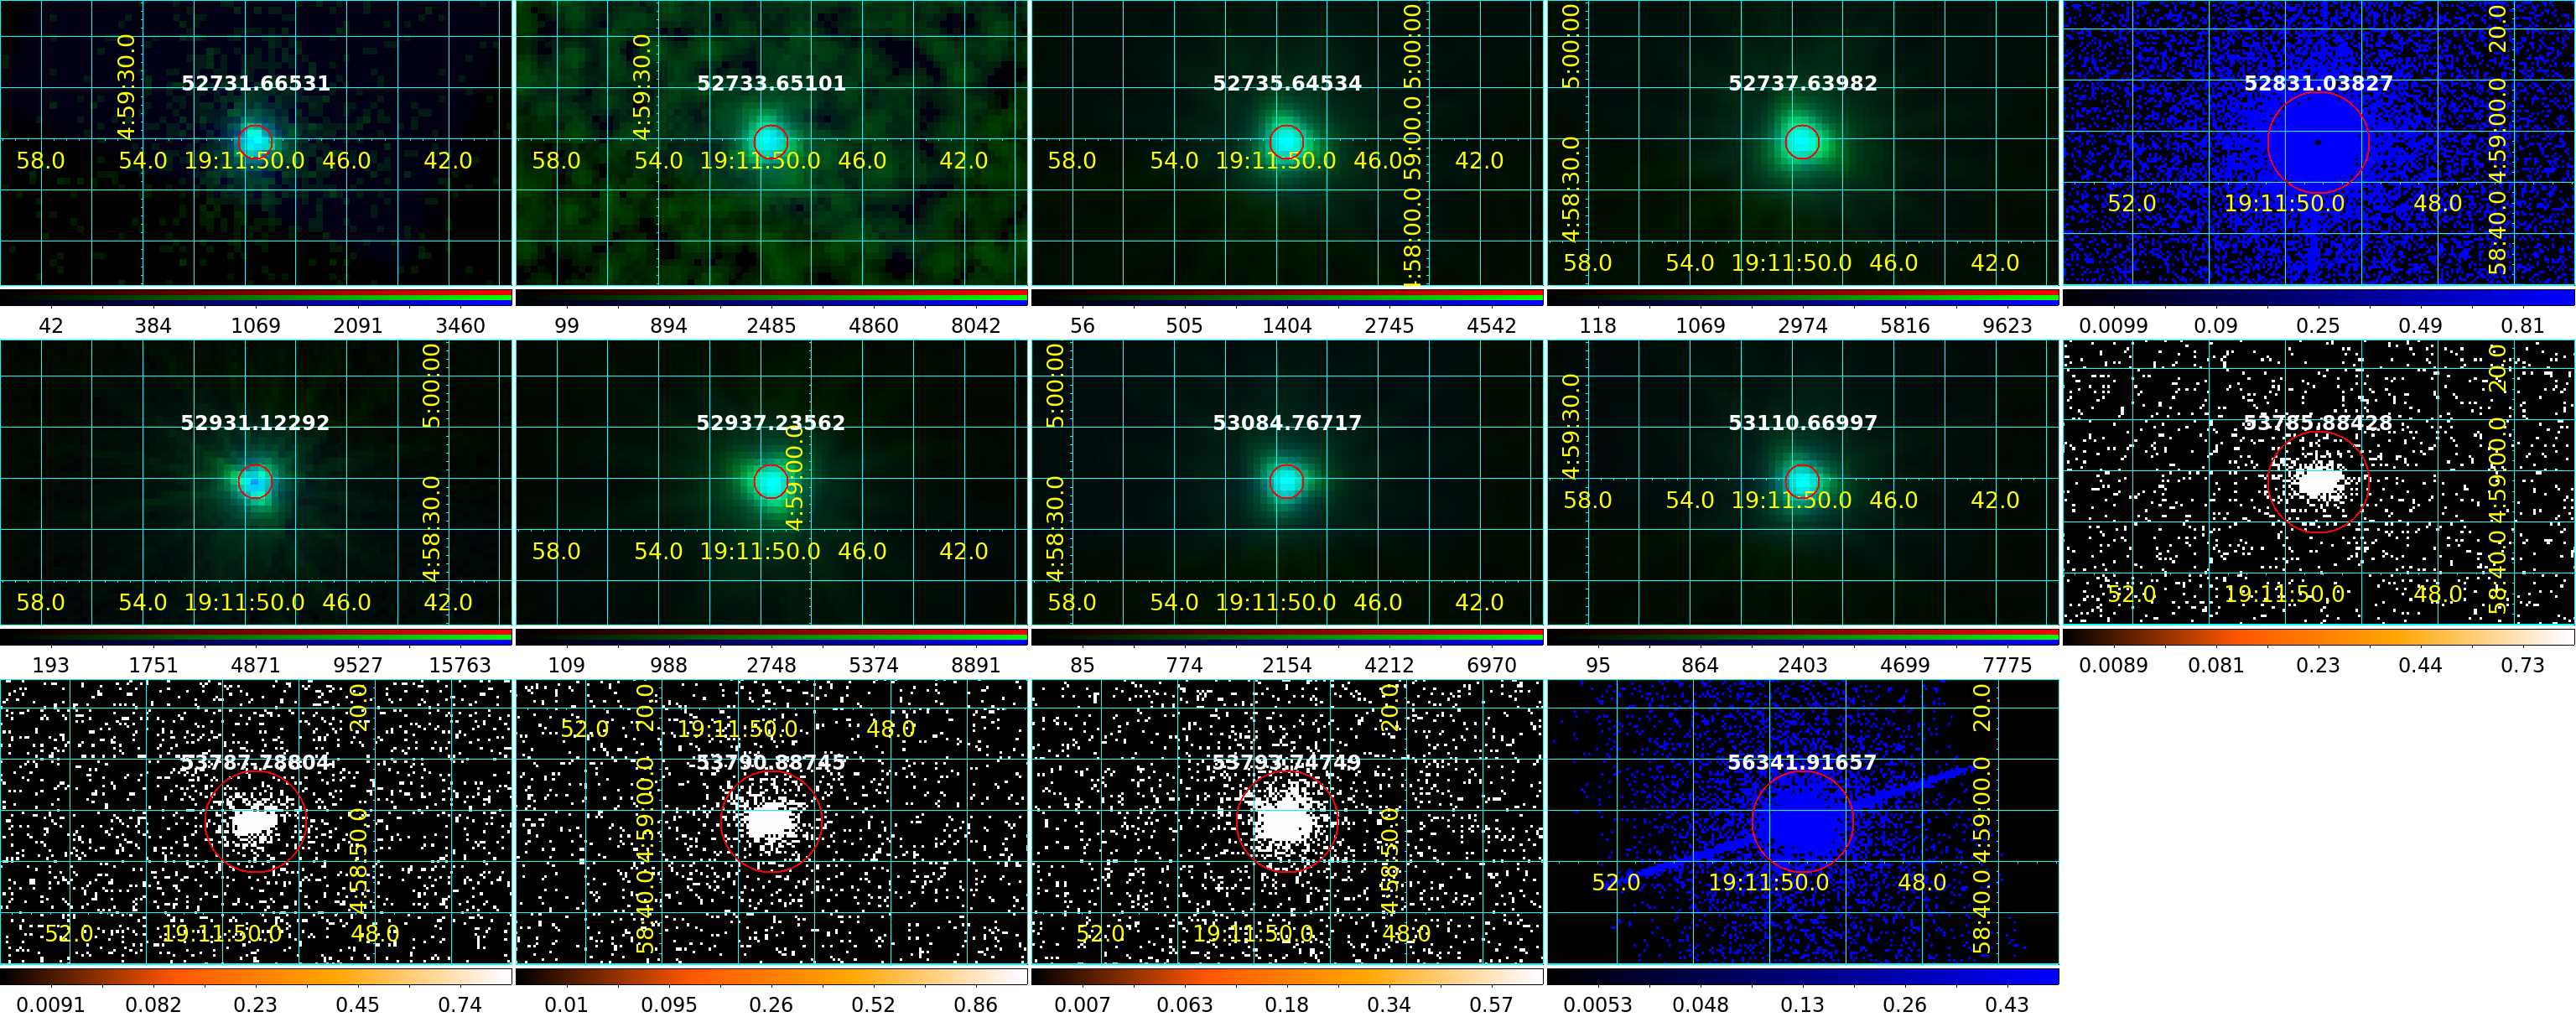
\includegraphics[width=0.97\linewidth]{figs/ss433}\\[8pt]
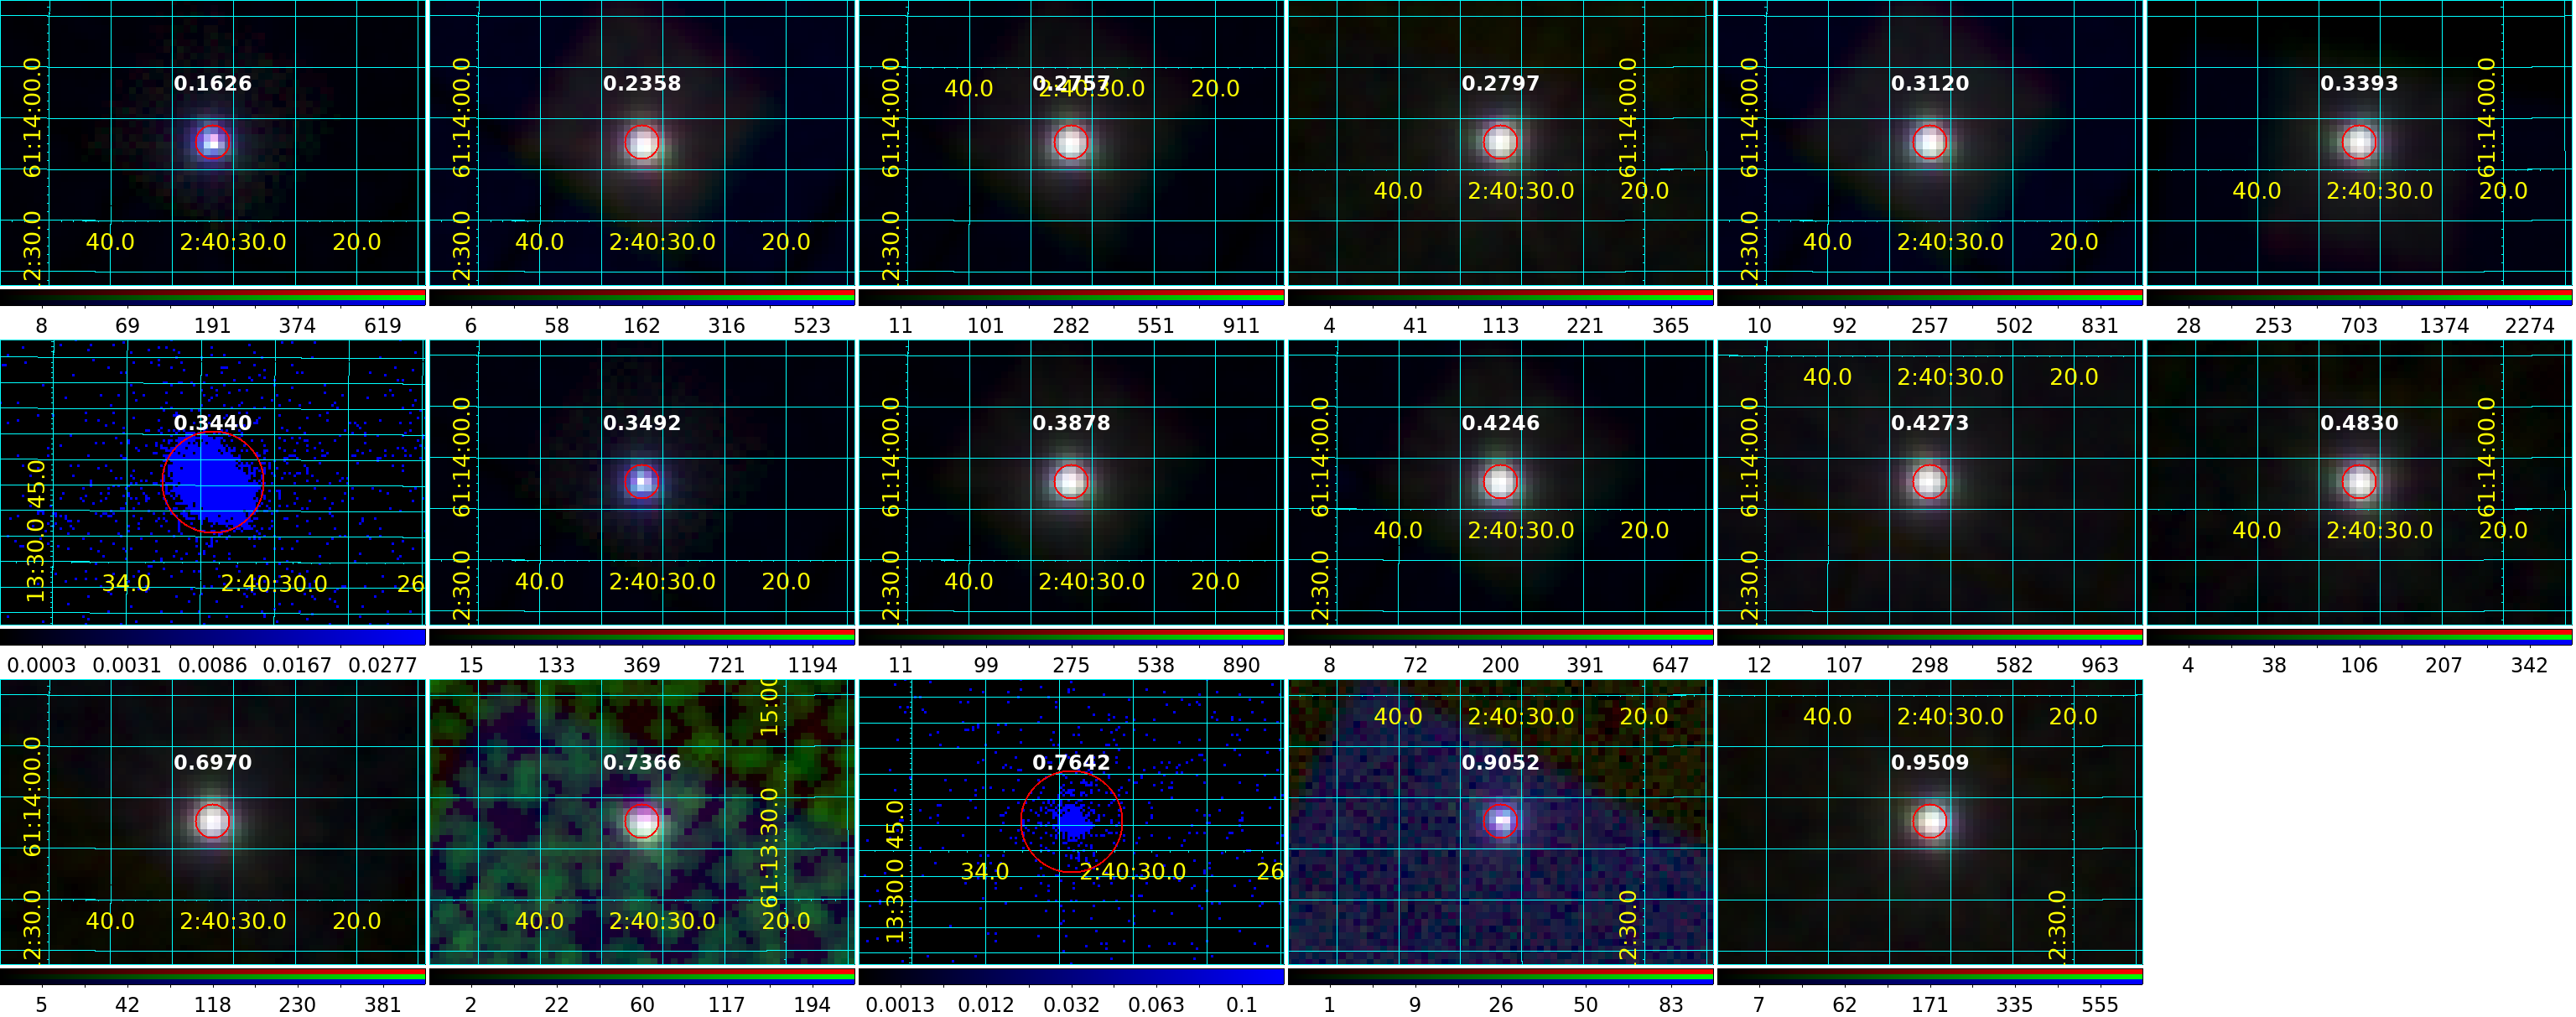
\includegraphics[width=0.97\linewidth]{figs/lsi61303}\\[8pt]
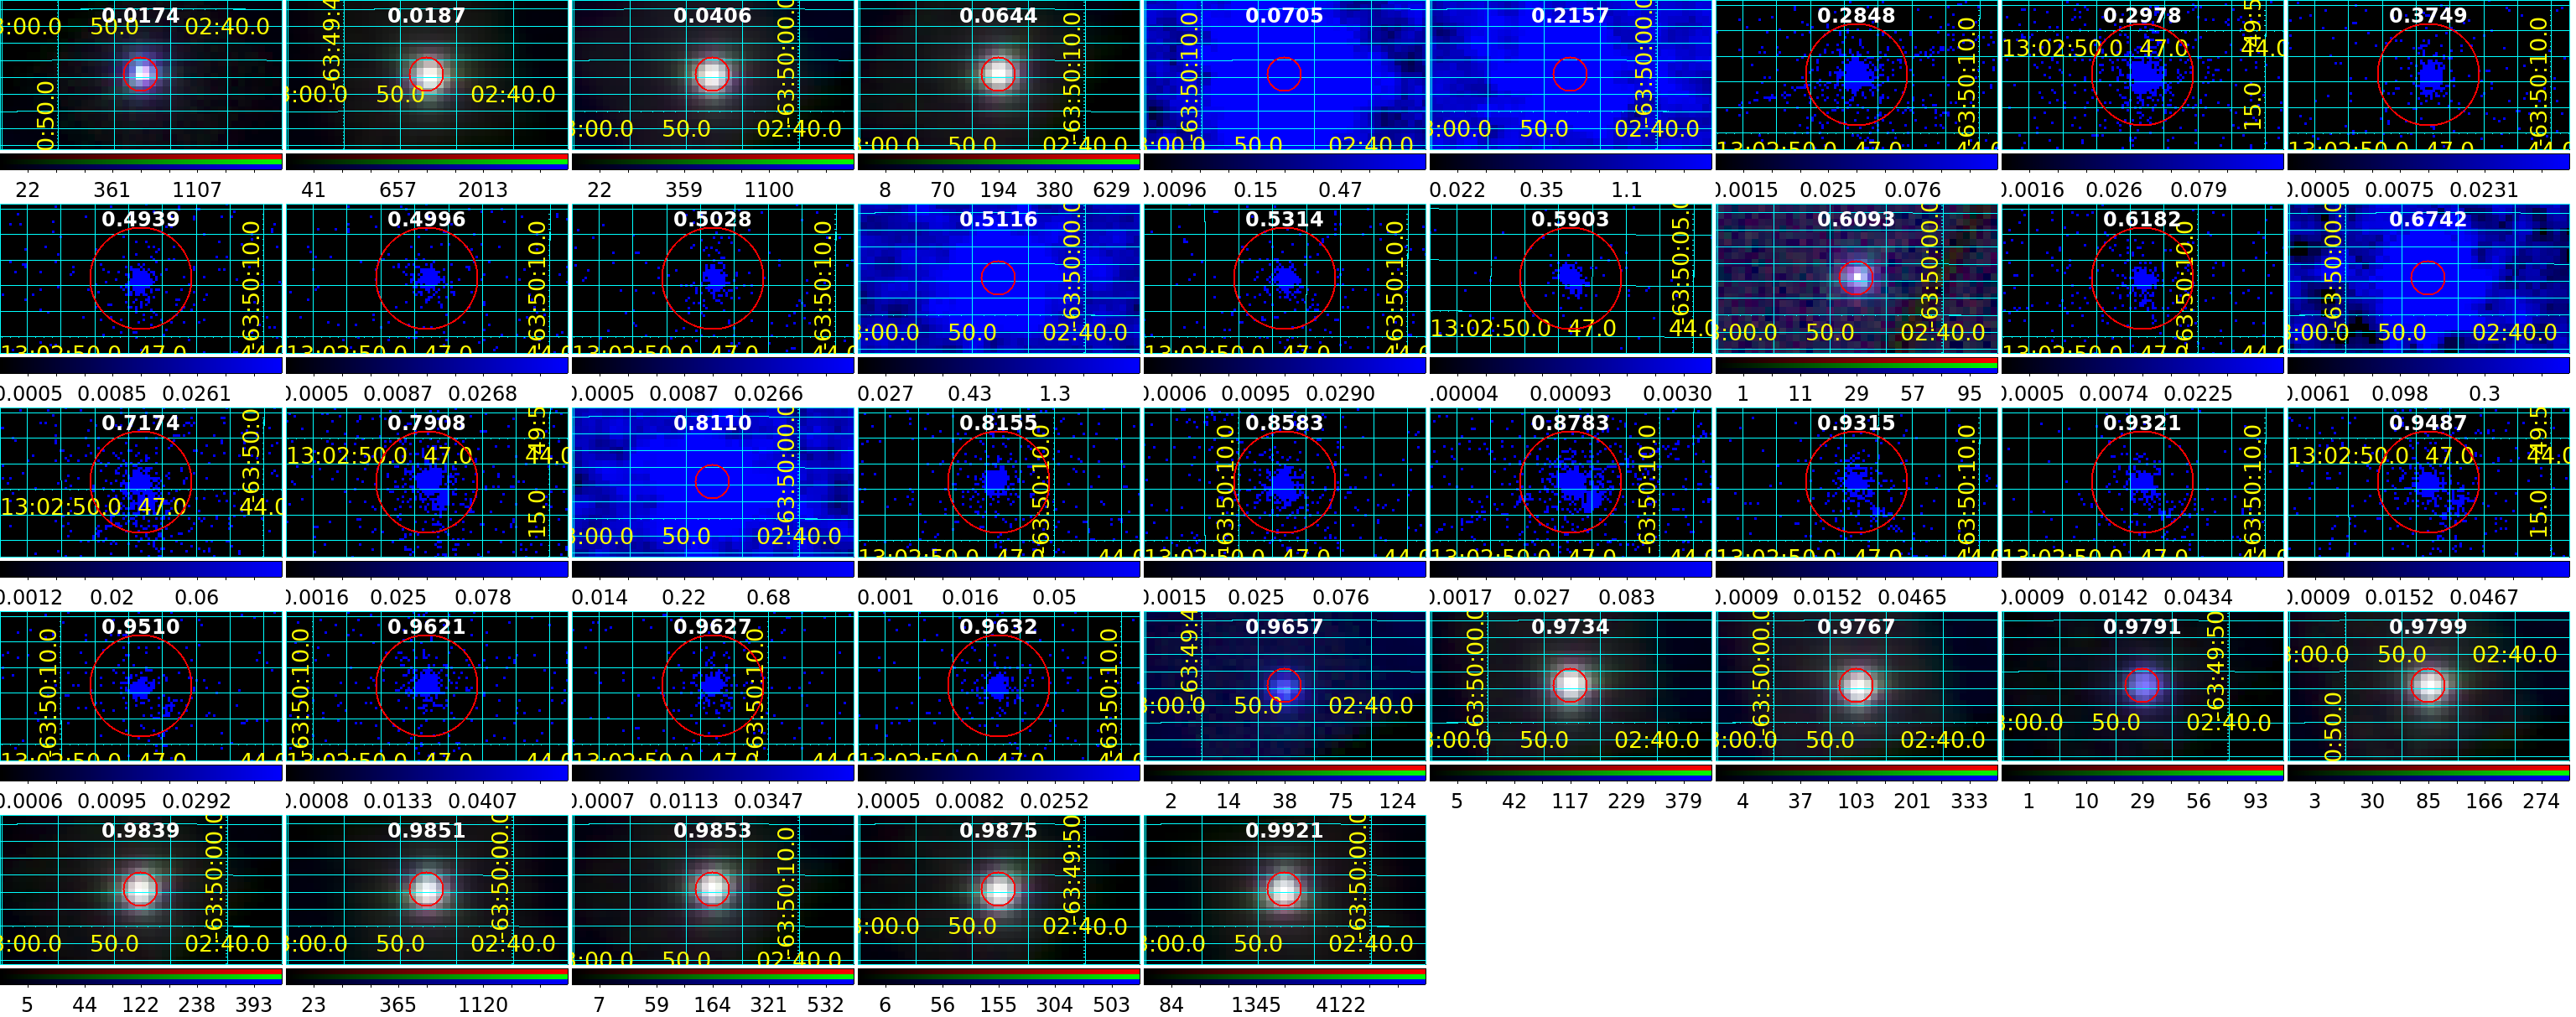
\includegraphics[width=0.97\linewidth]{figs/psrb1259}
\caption{Mosaics from the ds9 driver, each saved with one command. Top to
bottom: SS~433, 14 observations in time order; LS~I\,$+61^{\circ}$303, 17 in
phase order; PSR~B1259$-$63, 41 in phase order. A tile is one observation,
centred on the source and marked with a $10''$ circle, the number above it being
the phase or the MJD. The colour scale is raw counts per image pixel,
uncorrected for exposure or vignetting, square-root stretched to the 99.5th
percentile \emph{of that tile alone}, so each bar carries its own limits and
brightness is not comparable between tiles. In a three-colour tile red, green
and blue are the counts of EMOS1, EMOS2 and EPN, each scaled on its own data.}
\label{fig:mosaics}
\end{figure}

\end{document}
